Im vorherigen Kapitel haben wir gesehen, welche Zahlen in einem Fliesskommazahlensystem dargestellt werden können, das heisst welche Zahlen  exakt in einem Computer gespeichert werden können. Alle andere Zahlen werden gerundet. Computer werden aber nicht nur zum Speichern von Zahlen verwendet, sondern auch für Berechnungen.  Auch bei Berechnungen verhalten sich Fliesskommazahlen nicht ganz wie reelle Zahlen. In diesem Kapitel werden wir dies am Beispiel der Addition erfahren. 

\begin{beispiel}
Wir möchten \(1/4 + 1/8\) ausrechnen. Der erste Schritt ist beide Zahlen als Fliesskommazahlen aufzuschreiben. Wie in den vorherigen Kapiteln, sind in violett die reelle Zahlen in Basis 2 aufgeschrieben und braune ''Kasten'' mit orangenem ''Seil'' verwendet, um Mantisse und Exponent zu veranschaulichen. Rechts wird das Bitmuster in der gewöhnlichen Form angegeben.
\begin{figure}[H]
\centering
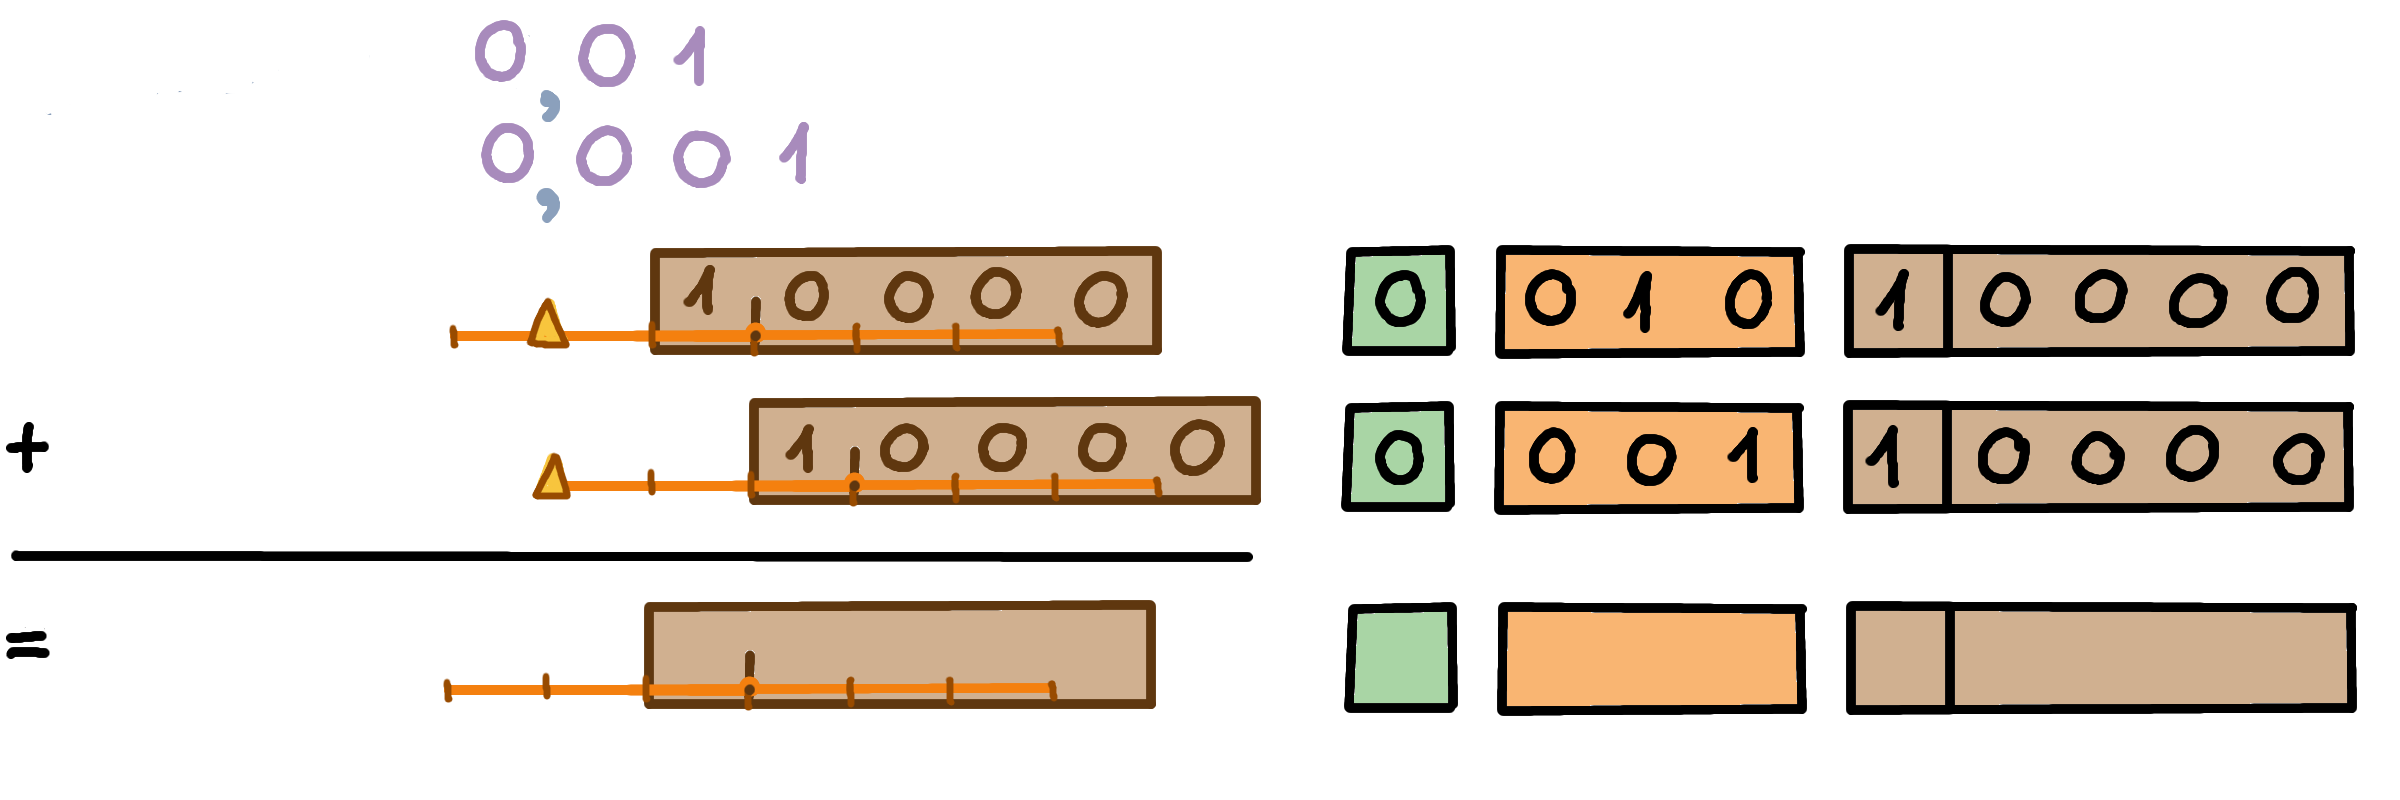
\includegraphics[width=\linewidth]{Pictures/Addition1-4and1-8_1.png}
\end{figure}

Damit wir die Bits der Mantisse stellenweise addieren können, wie wir das von den ganzen Zahlen kennen, müssen wir die zwei ''Kasten'' so verschieben, dass sie sich untereinander befinden. Da alles, was ausserhalb vom ''Kasten'' landet, verloren geht, werden wir den Kasten von der kleineren Zahl unter den Kasten von der grösseren Zahl schieben. So werden wir die Stellen mit dem niedrigsten Wert verlieren. In diesem Fall verlieren wir eine Null, der Wert der Zahl verändert sich also nicht.

Beachte, dass wenn der Kasten verschoben wird, verschiebt sich auch die Markierung bezüglich des ''Seils'', das heisst der Exponent verändert sich. Die Markierung am ''Seil'' bleibt immer unter dem Komma.
\begin{figure}[H]
\centering
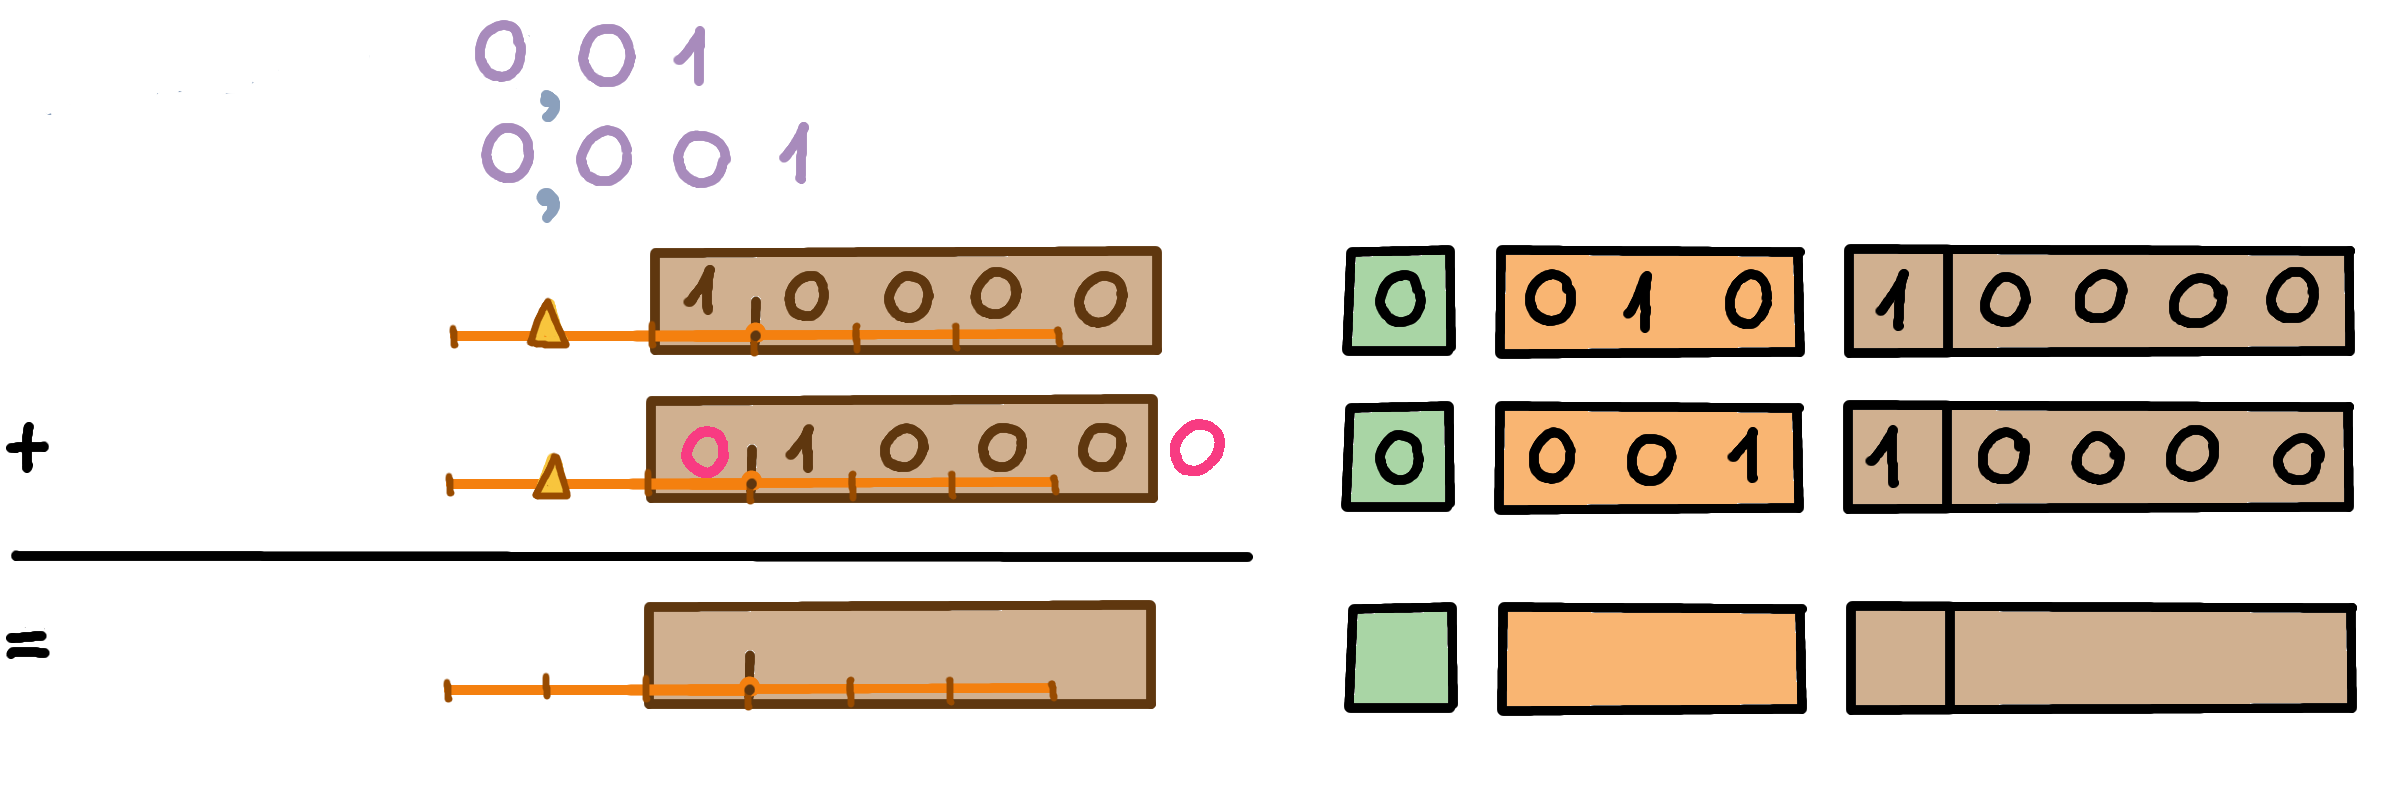
\includegraphics[width=\linewidth]{Pictures/Addition1-4and1-8_2.png}
\end{figure}

Wenn die Kasten untereinander sind, können wir die Bits in den Kasten wie gewöhnlich addieren, wie bei den Integers.
\begin{figure}[H]
\centering
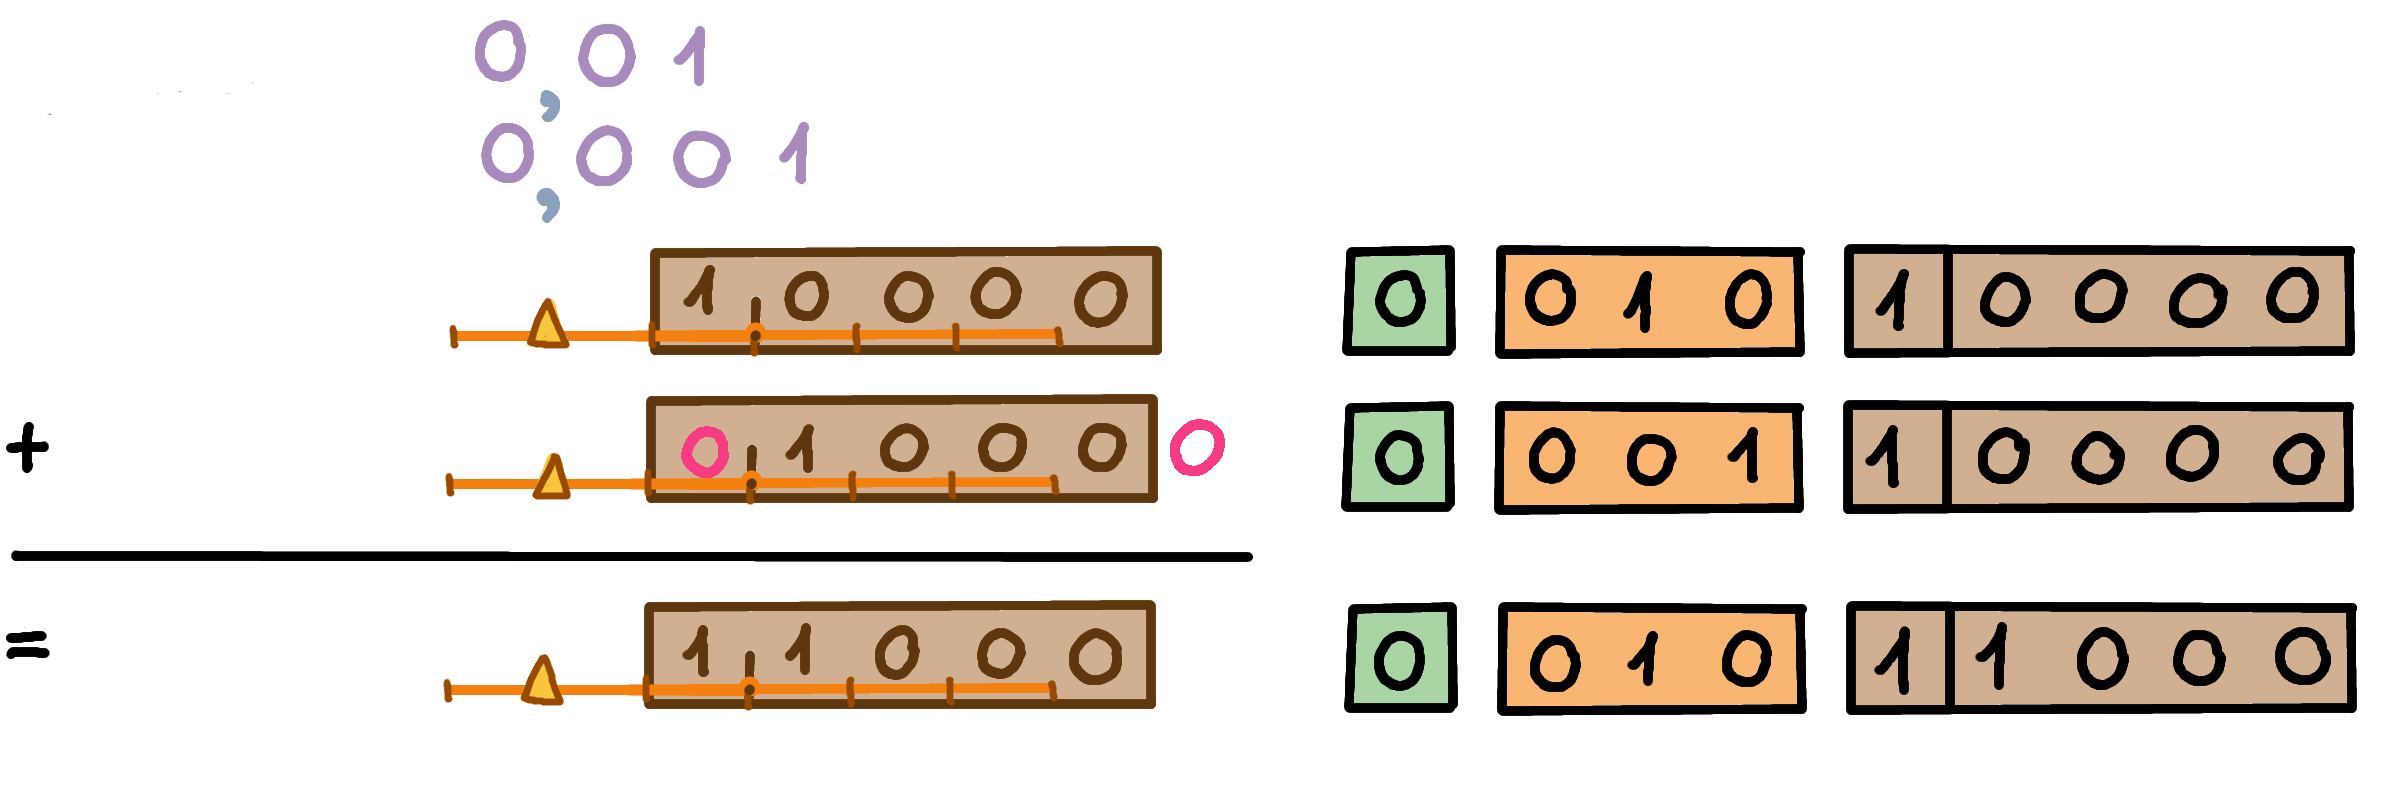
\includegraphics[width=\linewidth]{Pictures/Addition1-4and1-8_3.png}
\end{figure}
Wir haben ausgerechnet, dass \(1/4 + 1/8 = 3/8\), in der Exponentialschreibweise \(1.1000 \cdot 2^{-2}\).
\end{beispiel}

\begin{beispiel}
Wir möchten \(2+3\) ausrechnen. Im ersten Schritt schreiben wir beide Zahlen auf.
\begin{figure}[H]
\centering
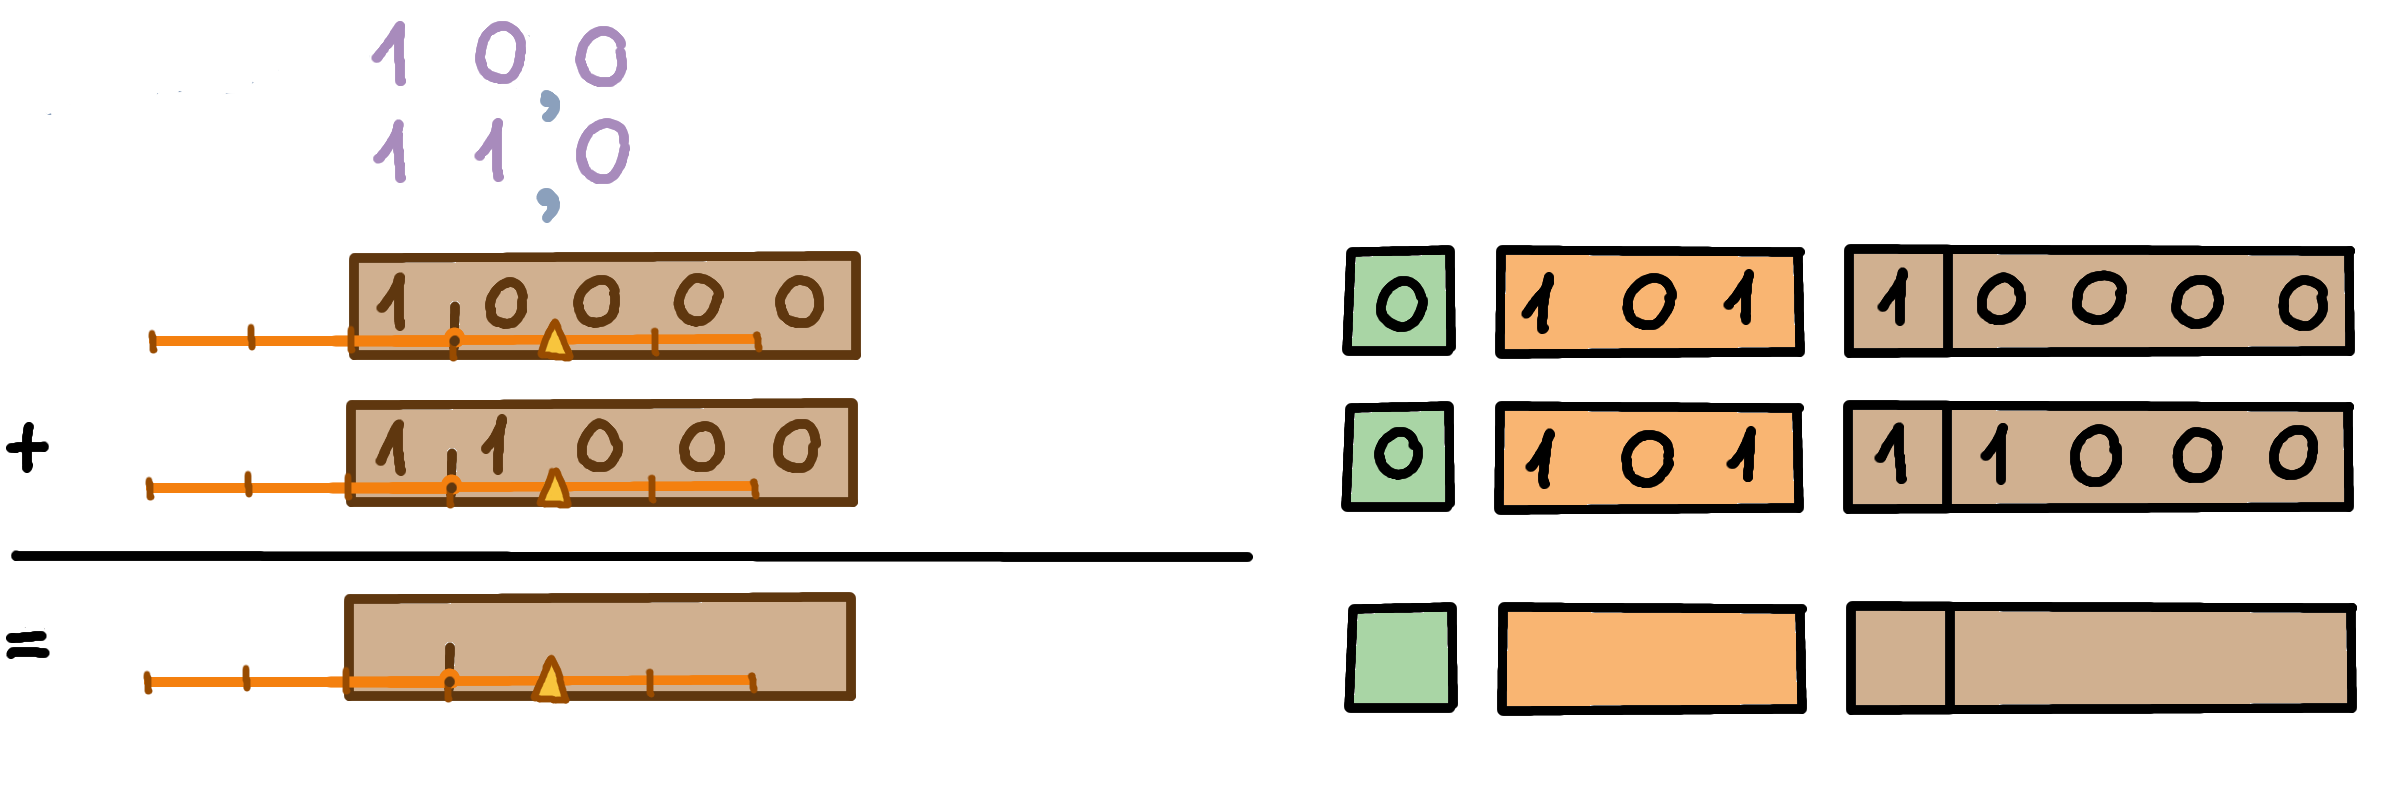
\includegraphics[width=\linewidth]{Pictures/Addition2and3_1.png}
\end{figure}
Die Kasten befinden sich schon untereinander. Wir müssen also nichts verschieben und können sofort losrechnen.
\begin{figure}[H]
\centering
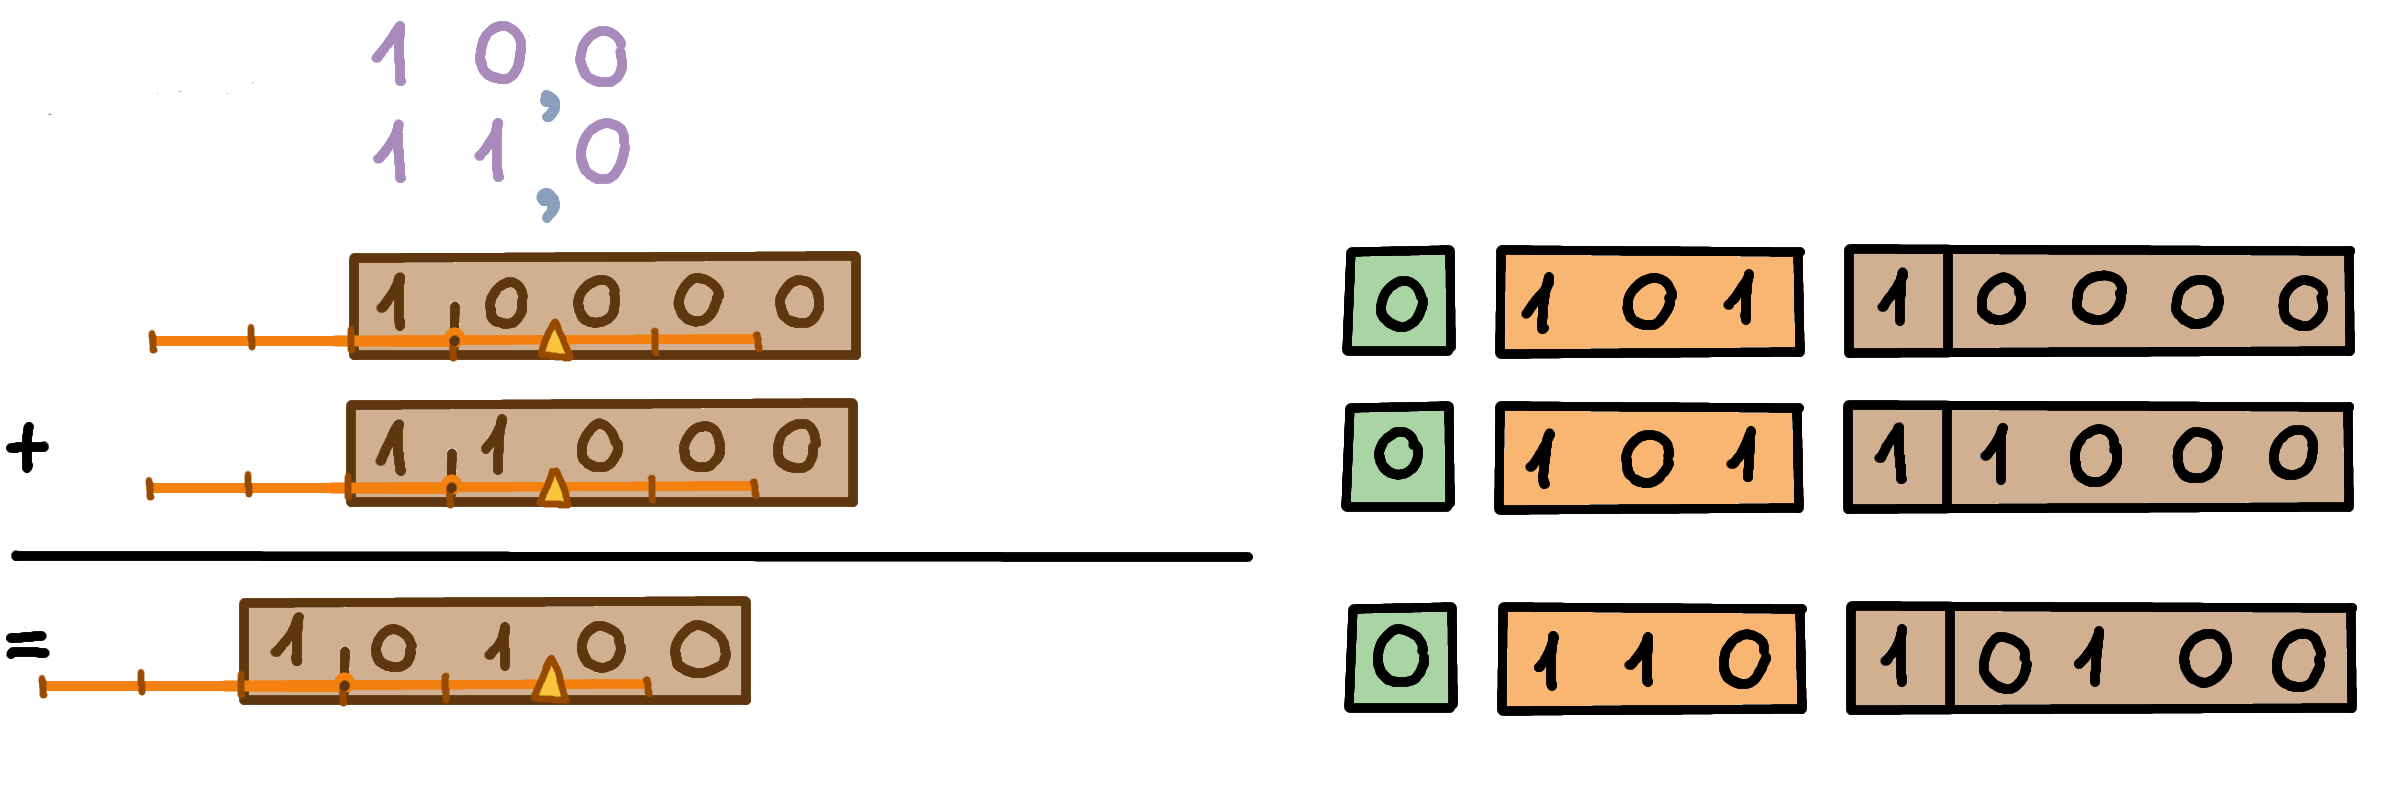
\includegraphics[width=\linewidth]{Pictures/Addition2and3_2.png}
\end{figure}
Beachte, dass der Kasten vom Ergebnis bezüglich den Kasten der Summanden verschoben ist, um die neue signifikante Stelle zu enthalten.

Wir haben ausgerechnet, dass \(2 + 3 = 5\), in der Exponentialschreibweise \(1.0100 \cdot 2^2\).
\end{beispiel}

\begin{aufgabe}\label{addition}
Rechne folgende Summen aus. Die Mantissenlänge beträgt \(5\) Bits, der Exponent geht von \(-3\) bis \(3\). Gebe bitte das Bitmuster und die Exponentialdarstellung des Resultats an.
\begin{enumerate}[(a)]
\item \(5/8 + 3/4\)
\item \(10 + 2.25\)
\item \(17/16 + 2\)
\end{enumerate}
\end{aufgabe}

Die Addition im Fliesskommazahlensystem ist wie gewöhnlich kommutativ, weil wir immer die kleinste Zahl so verschieben, dass ihr Kasten unter dem Kasten der grösseren Zahl steht und dann die Bits in beiden Kasten stellenweise zusammen addieren.

\begin{aufgabe}\label{lernaufgabe_assoziativ}
Berechne dazu zwei Mal die gleiche Summe in einem Fliesskommazahlensystem mit Mantissenlänge \(5\) und Exponenten von \(-3\) bis \(3\):
Das erste Mal als \(1/8 + 2/8 + 3/8 + 4/8 + 5/8 + 6/8 + 7/8 + 8/8\) und das zweite Mal als \(8/8 + 7/8 + 6/8 + 5/8 + 4/8 + 3/8 + 2/8 + 1/8\).

Welchen Resultat erwartest du? Sind die zwei Summen gleich oder unterschiedlich?
Nimm dir Zeit und rechne die zwei Summen tatsächlich aus.
\end{aufgabe}

Die zwei Summen, die du ausgerechnet hast, liefern unterschiedliche Ergebnisse. Die erste liefert den exakten Wert \(4.5\), während bei der zweiten Summe kriegen wir im Fliesskommazahlensystem nur \(4.25\), und das obwohl der exakte Wert dargestellt werden kann. Das passiert, weil man bei den Fliesskommazahlen nur Zahlen der ähnlichen Grössenordnung exakt addieren kann. In der ersten Summe addieren wir die kleineren Summanden am Anfang, wenn die kumulative Summe noch nicht zu gross ist. In der zweiten Summe wächst die kumulative Summe sehr schnell, und irgendwann sind die Summanden zu klein bezüglich der kumulativen Summe, um einen Unterschied zu machen.

Daraus können wir folgern, dass die Addition bei den Fliesskommazahlen nicht assoziativ ist.


\begin{aufgabe}\label{ein_achtel}
Betrachten wir die Summe \(1/8 + 1/8 + 1/8 + \dotsb + 1/8\).
Bei den reellen Zahlen können wir mit solchen Summen auf beliebig grossen Zahlen kommen. Bei den Fliesskommazahlen kann das nicht gehen, weil, wie wir im vorherigen Kapitel gesehen haben, es eine grösste Fliesskommazahl gibt. Aber können wir diese Zahl auch tatsächlich erreichen?

In einem Fliesskommazahlensystem mit Mantissenlänge \(5\) und Exponentenbereich von \(-3\) bis \(3\), was ist die grösste Zahl, die wir erreichen können, wenn wir beliebig viele \(1/8\) zusammen rechnen? Wie viele Summanden brauchen wir, um diese Zahl zu erreichen?
\end{aufgabe}


\subsubsection*{\textcolor{blue-violet}{Teste dich selber}}
\begin{aufgabe}\label{addition_kontrollfragen}
Beantworte folgende Fragen:
\begin{enumerate}[(a)]
\item Warum kann man im Allgemeinen zwei Mantissen nicht stellenweise zusammen addieren?
\item Gregory behauptet, dass der Kasten vom Ergebnis sich immer genau unter dem Kasten der grössten Zahl befindet. Hat er recht? Argumentiere.
\item Hannah behauptet, dass die Addition bei den Fliesskommazahlen nicht kommutativ und nicht assoziativ ist. Hat sie recht? Argumentiere.
\end{enumerate}
\end{aufgabe}

\begin{aufgabe}\label{ameisenkönigin}
Die Ameisenkönigin möchte ausrechnen, wie viele Ameisen braucht sie, um \(10\) Reiskörnchen zu transportieren. Sie weiss, dass eine Ameise allein \(1/4\) Reiskorn transportiert. Die Ameisenkönigin hat dazu folgendes Programm geschrieben.
\begin{lstlisting}[language=Python, caption={Programm von der Ameisenkönigin}]
def nof_ameisen():
    sum = 0.0
    i = 0
    while node != 10.0:
    	i += 1
       sum += 0.25
    return i
\end{lstlisting}
Die Ameisencomputer arbeiten mit Fliesskommazahlen mit Mantissenlänge \(5\) und Exponenten zwischen \(-3\) und \(3\).
Kann die Ameisenkönigin mit diesem Programm die gewünschte Anzahl Ameisen herausfinden? Falls ja, wie viele Ameisen braucht sie, um 10 Reiskörnchen zu transportieren laut diesem Programm? Falls nein, was ist die maximale Summe, die das Programm erreichen kann?
\end{aufgabe}